\chapter{生成式設計}
運用電腦輔助系統的創造工具,利用軟體設計出所需的3D模型,輸入的參數或製作、預期要求,將成品利用電腦算法,強大的運算會模擬許多所有可能性及排列,並產生多個解決方案。\\
主要依靠人工智能和機器學習來模仿自然界的進化設計方法,創造出許多種可能性,
利用AI運算生成整合並優化零件,創造出可能從未發現的幾何圖形,將產品創新優化,讓零件在輕盈的狀況下還保有堅韌程度,最大程度減低所需要耗費的人力、時間成本,讓成品可以快速並有效的產出。\\

%-----------------------生成式設計原理-------------------------%
\section{生成式設計原理}
生成式設計是一個迭代設計過程,透過軟體多次的分析與設計,生成符合製作條件的模型設計。生成式設計是一種電腦輔助設計的方法,利用軟體的AI智能算法,將設計者輸入的模型設計條件進行多次生成,並尋找出最佳設計。
生成式設計的主要功用為優化零件,不只能夠設計出更輕量化的零件,並且也能使各項性質提升,像是強度更強、更耐用、散熱快等。\

%-----------------------設計流程-------------------------%
\section{設計流程}
\begin{itemize}
\item 定義問題:確定設計問題的範圍和目標
\item 創建設計規則:定義出用來生成設計方案的規則和條件。
\item	建立生成系統:選擇合適的軟體,利用AI生成設計。
\item 優化生成結果:當生成設計方案後,進行評估和優化,並對設計方案進行手動調整或修改,以便滿足特定的要求。
\end{itemize}

%-----------------------零件優化-------------------------%
\section{零件優化}
為了將零件輕量化,並維持其原本的零件強度,我們透過Solid Edge軟體將零件進行生成式設計,經過軟體的AI迭代算法以及多次修改設計參數,最後選擇最符合實際的設計。\

\begin{figure}[htbp]
  \begin{minipage}[t]{0.5\linewidth}
    \centering
    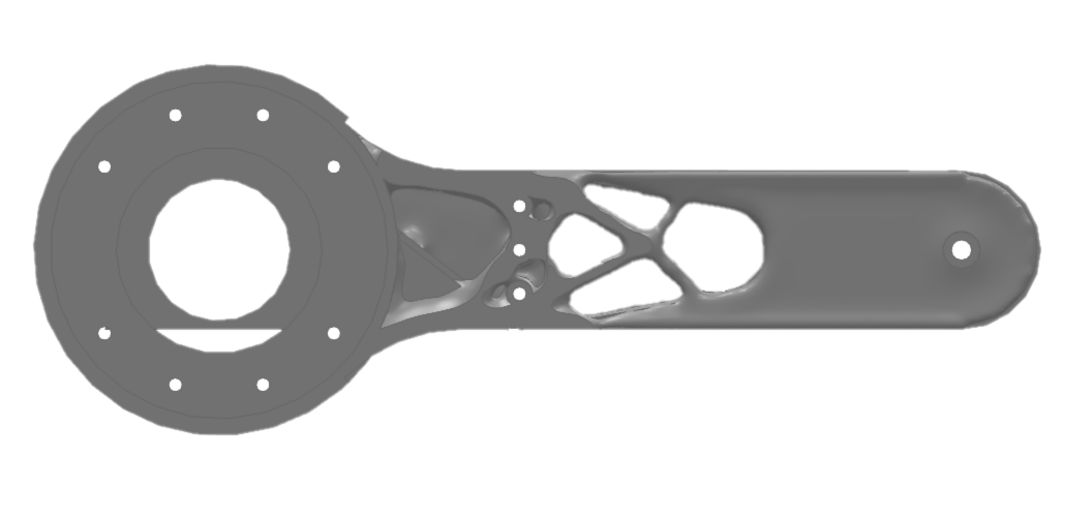
\includegraphics[height=6cm,width=6cm]{Leg1-1+1-5(拓樸)}
    \caption{leg1-1+1-5(生成)}
    \label{Leg1-1+1-5(拓樸)}
  \end{minipage}
  \hfill
  \begin{minipage}[t]{0.4\linewidth}
    \centering
    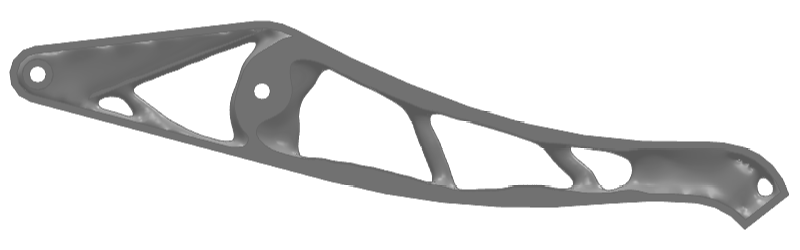
\includegraphics[height=6cm,width=6cm]{Leg4(拓樸)}
    \caption{leg4(生成)}
    \label{Leg4(拓樸)}
  \end{minipage}
\end{figure}
